\begin{center}
    

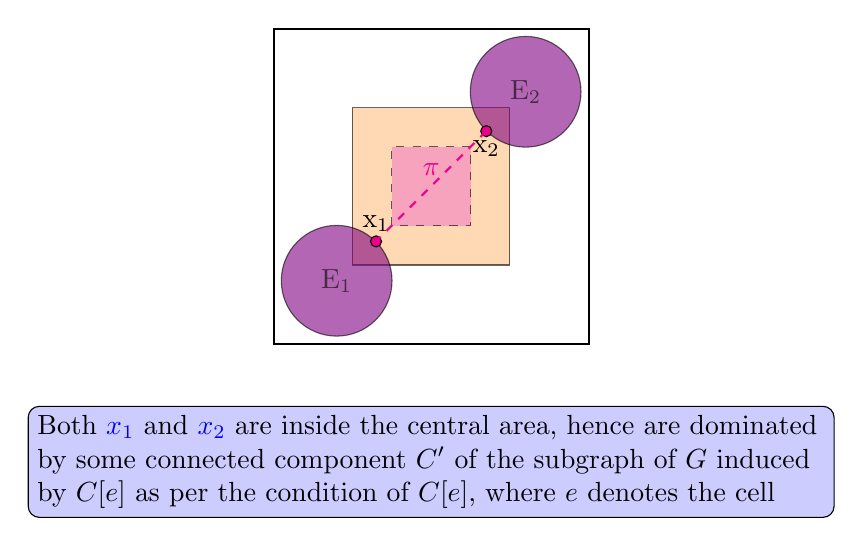
\begin{tikzpicture}

    % Square in the middle
    \draw[thick] (1, 1) rectangle ++(4, 4);
    \draw[fill=orange!50, opacity = 0.6] (2, 2) rectangle ++(2, 2);
    \draw[dashed, fill=magenta!50, opacity = 0.6] (2.5, 2.5) rectangle ++(1, 1);

    \filldraw[fill=violet, opacity = 0.6] (1.8, 1.8) circle (20pt) node {E$_1$};
    \filldraw[fill=violet, opacity = 0.6] (4.2, 4.2) circle (20pt) node {E$_2$};

    \filldraw[fill=magenta] (3.7, 3.7) circle (2pt) node[below] {x$_2$};
    \filldraw[fill=magenta] (2.3, 2.3) circle (2pt) node[above] {x$_1$};

    \draw[thick, dashed, magenta] (3.7, 3.7) -- (2.3, 2.3) node[above, midway]{\textbf{$\pi$}};

    \node[draw, fill=blue!20, text width=10cm, rounded corners] at (3, -0.5) {
    Both \textcolor{blue}{$x_1$} and \textcolor{blue}{$x_2$} are inside the central area, hence are dominated by some connected component $C^\prime$ of the subgraph of $G$ induced by $C[e]$ as per the condition of $C[e]$, where $e$ denotes the cell  
    };
    
     

\end{tikzpicture}

\end{center}